\section{The Large Hadron Collider}
\label{sec:lhc}

\subsection{CERN complex}

\onehalfspacing CERN accelerator complex is a progression of machines namely Linac 2, Proton Synchrotron Booster (PSB), Proton Synchrotron (PS), Super Proton Synchrotron (SPS) and Large Hadron Collider (LHC) as shown in Fig. 3 that accelerate particles mainly protons to increasingly higher energies of 50 MeV, 1.4 GeV, 25 GeV, 450 GeV and 14 TeV respectively \cite {CERNBrochure2017002Eng}. Each machine is used to increase the energy of particle before the beam is injected into to the next machine. Linear accelerator (Linac2) is the starting point for protons used in various experiments at CERN. After proton energy reaches 50 MeV, protons enter PSB which further increases its energy before they are injected into PS which takes up its energy to 25 GeV. After reaching 25 GeV, protons enter SPS which further increases its energy to 450 GeV. The protons are finally transferred to two beam pipes of LHC kept at very high vacuum to collide at the interaction points and then proton beam is dumped after sometime (1-35 hours). This entire procedure defines a single LHC fill generally consisting of $10^{14}$ protons, grouped into bunches to form the proton beam as shown in Fig. 4. \\ 

The Large Hadron Collider (LHC) is the most powerful particle accelerator in the world primarily build to collide protons and heavy ions at 7, 8, 13 and 14 TeV during different LHC run period. The LHC consists of a 27 km ring of superconducting magnets producing strong magnetic field which is used to guide particle beams along the LHC ring. Proton beam is made up of bunches travelling in opposite directions kept in two ultrahigh vacuum tubes are accelerated close to the speed of light using time dependent electric field produced by radiofrequency cavities before they collide at four interaction points along the LHC ring where ATLAS, ALICE, CMS and LHCb detectors are placed \cite {CERNBrochure2017002Eng}. \\


\begin{figure}[H]
  \centering
  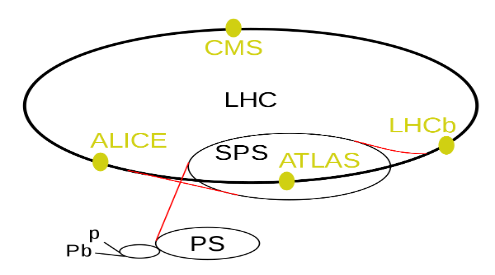
\includegraphics[width=0.8\columnwidth]{./LHCcomplex.png}
  \caption{\onehalfspacing Diagram of the LHC accelerator complex located in Geneva, Switzerland. Four interaction points are shown where the ALICE, ATLAS, LHCb and CMS detectors are stationed \cite{Mobs:2684277}.}
  \label{fig:LHC}
\end{figure}


\begin{figure}[H]
  \centering
  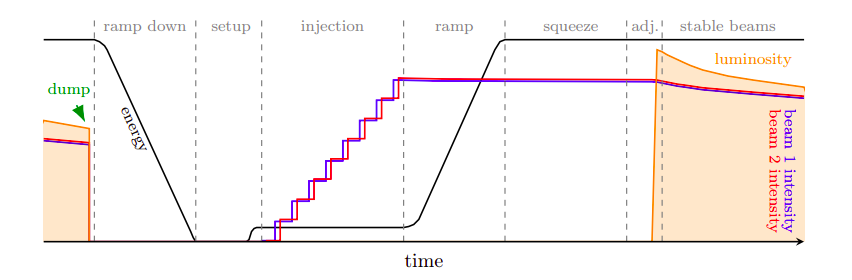
\includegraphics[width=1 \columnwidth]{./lhcfill.png}
  \caption{ \onehalfspacing A typical operational LHC cycle which involves set up (beam is accepted from injector complex), injection (beam is injected into LHC ring in form of bunch train), ramp (current in dipole increased to reach highest energy), squeeze (bunches are squeezed to have minimum proton separation in them), adjust (separation between beams at the interaction point is removed) and stable beams (collision settings are invoked and data taking period starts) \cite{fill}.}
  \label{fig:LHCPlans}
\end{figure}

\subsection {Run 1 and 2 of LHC}
The first proton beam was successfully maneuvered around the LHC ring in September 2008 that marked the beginning of Run 1 with proton beams colliding at 7-8 TeV center-of-mass energy and this run period ended in 2013 \cite{cmsrun} \cite{Alemany-Fernandez:1631030}. Run 2 started in 2015 with protons colliding at 13 TeV center-of-mass energy and continued till October 2018 \cite{Wenninger:2668326}. Run 3 is expected to begin at the start of March 2022 and High Luminosity (HL)-LHC phase is expected to begin in mid-2027 \cite{Dainese:2019rgk}. Proton Synchroton (PS) is responsible for providing proton bunches spaced 7 metres (25 ns) apart with each bunch containing more than 100 billion protons as shown in Fig. 5. The maximum number of bunches reached with the beam preparation method used during Run 2 is 2556 \cite{Wenninger:2668326}. The number of protons in the colliding bunches, time of separation between the bunches and effective area of the bunch which depend on the rms transverse bunch size along horizontal and vertical directions as shown in Fig. 6 is one of the ways to calculate instantaneous luminosity $(L_{inst})$. The number of proton proton collisions per bunch crossing is called pileup ($\mu$).\\

Rate of collision = $\sigma$ L = $(60 mb) (7.5 $\times$ 10^{34} cm^{-2} s^{-1})$ = $(60 $\times$ 10^{-3} $\times$ 10^{-24}) (7.5 $\times$ 10^{34})$ = 6000 million/s \\ 

where $1 \:barn = 10^{-24} cm^2$ and $1 \:mb = 10^{-27} cm^2$.\\

Colliding bunch rate = number of colliding bunches $\times$ LHC revolution frequency = 2800 $\times$ 11246\:Hz = 28.7\:MHz = 31.4 \:million/s \\

Pileup ($\mu$) = $\frac{Rate \:\:of \:\:collision}{colliding \:\:bunch\:\: rate} = \frac{6000 \:million/s}{31.4 \:million/s}$ = 200   for HL-LHC.    \\


\begin{figure}[H]
  \centering
  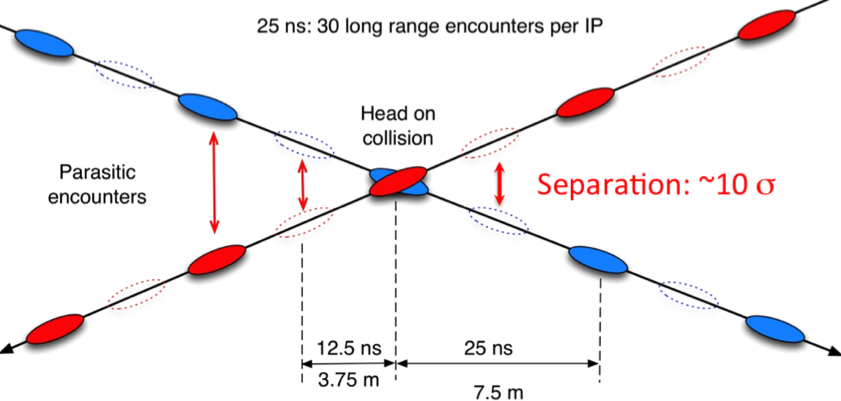
\includegraphics[width=0.6\columnwidth]{./LHCReport_1_image_cut.png}
  \caption{ \onehalfspacing Diagram showing colliding bunches in each LHC beam separated by 25ns.}
  \label{fig:CMS}
\end{figure}


\begin{figure}[H]
  \centering
  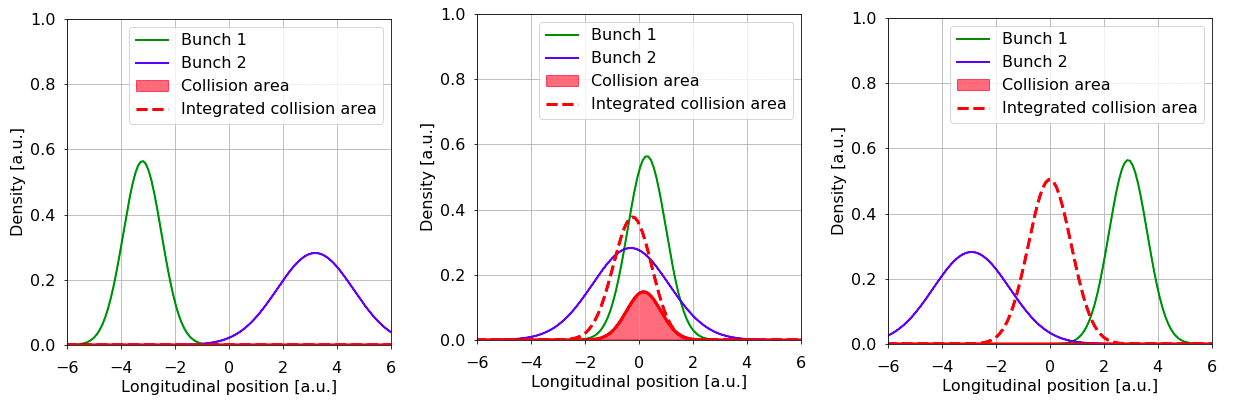
\includegraphics[width=\columnwidth]{./vdm_image.png}
  \caption{\onehalfspacing Figure showing two LHC bunches in green and blue approaching each other and colliding giving rise to bunch overlapping region shown in red.}
  \label{fig:CMS}
\end{figure}



\subsection{Luminosity and Phase II HL-LHC}
Luminosity is a key performance parameter of an accelerator as it is a measure of number of collisions. Luminosity can be categorized into two types: instantaneous and integrated luminosity. Instantaneous luminosity corresponds to the number of collisions occuring per second in per centimeter square area while integrated luminosity is obtained by integrating instantaneous luminosity over a time interval. Both are very important variables as they are used to obtain the number of collision events. During Run 1, peak value of LHC instantaneous luminosity was $0.77 \times 10^{34} \: cm^{-2} s^{-1} $ with $30 \: fb^{-1}$ integrated luminosity \cite{cmsrun1lumi}. During Run 2, LHC instantaneous luminosity reached a peak value of $2.1 \times 10^{34}  \: cm^{-2} s^{-1}$ with $163 \: fb^{-1}$ integrated luminosity as shown in Fig. 7 \cite{CMS:2018elu}. At the end of Run 3, we expect to achieve an integrated luminosity of $300 \:fb^{-1}$ while Phase II HL-LHC is expected to collect $3000 \:fb^{-1}$ of data as shown in Fig. 8 thereby increasing luminosity by a factor of 10 beyond the LHC's design value \cite{Dainese:2019rgk}. \\



\begin{figure}[H]
  \centering
  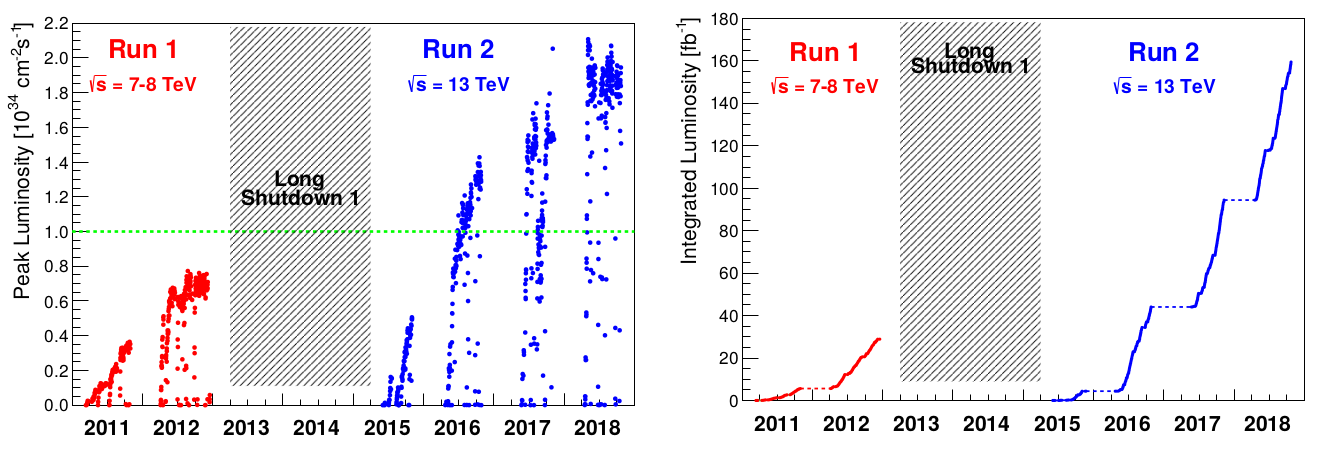
\includegraphics[width=1 \columnwidth]{./peakintlumi_run12.png}
  \caption{\onehalfspacing Left: Instantaneous luminosity for Run 1 and Run 2 period. Right: Integrated luminosity for Run 1 and Run 2 period \cite{lumi}.}
  \label{fig:LHClumi}
\end{figure}


\begin{figure}[H]
  \centering
  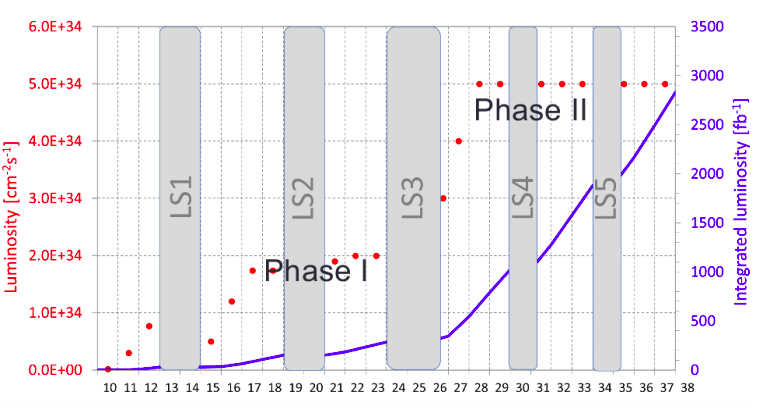
\includegraphics[width=0.7 \columnwidth]{./lumi_projection.png}
  \caption{ \onehalfspacing Projected performance of the LHC until 2038, which shows the preliminary dates for prolonged stops (LS1, LS2, LS3, LS4, LS5) of the LHC and luminosities. Red points show instantaneous luminosity $(L_{inst})$ while the blue line shows integrated luminosity \cite{collaborations2019report}.}
  \label{fig:LHCPlans}
\end{figure}


\clearpage\newpage







